\documentclass{UCreport}
\usepackage{lipsum}
\usepackage{gensymb}
\usepackage{float}
\usepackage{graphicx} % Required for inserting images



%
%
%   To cite by author name, uncomment this line.
\usepackage[authoryear,comma,round]{natbib} 
%
%
%   To instead cite by number, uncomment this line.
%\usepackage[square,numbers,comma,sort&compress]{natbib} 


\begin{document}

%----------- Report information ---------

\logo{logos/UC.png}
\school{\textbf{School of Physical and Chemical Sciences}}
\course{\textbf{PHYS480}}
\student{\textbf{My Name}}
\supervisor{Dr Jane Doe}
\ttitle{Title of the report} %title of the file


%----------- Init -------------------
        
\buildmargins % display margins
\buildcover % create the front cover of the document


%------------ Declaration ----------------

\pagenumbering{roman}

\addcontentsline{toc}{section}{Declaration}
\declaration

I certify that content of this report was mostly my own work.
\\

My supervisor helped by proofreading the report and offering feedback. \\

Graduate students, X and Y, helped me understand ... \\

The derivation in section 3 was taken from ... \\

\vspace{2cm}
\begin{centering}
\textbf{\student}\par
\end{centering}

\newpage


%------------ Abstract ----------------

\addcontentsline{toc}{section}{Abstract}
\abstract

This is where the abstract goes. \\

This is the next paragraph.


\newpage


%------------ Contents pages ----------------


\toc % creates the table of contents


\addcontentsline{toc}{section}{List of Figures}
\listoffigures
\newpage
\addcontentsline{toc}{section}{List of Tables}
\listoftables
\newpage


%------------ Report body ----------------

\pagenumbering{arabic}


\section{Introduction}

\subsection{Part of introduction}
This is a test.

\newpage

\section{Next section}

This is another test. A plot is shown in Fig.~\ref{fig:plot}.

\begin{figure}[ht]
\centering
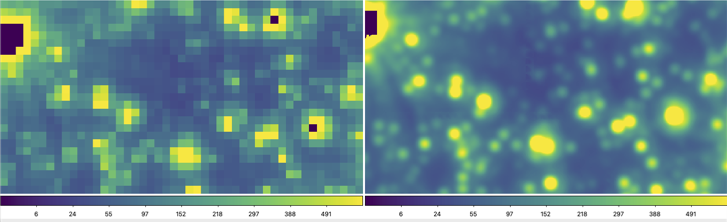
\includegraphics[width=0.8\textwidth]{figures/test_figure.png}
\caption{This is the caption.}
\label{fig:plot}
\end{figure}



As a citation test we can refer to \citet{Albrow2022} or use brackets (when using cite-by-name style) \citep{Hurley2005}.


Here is a table that we can refer to as Table~\ref{table:table1}.

\vspace{1cm}

\begin{table}[ht]
    \caption{Table captions go above.}
    \label{table:table1}
    \begin{tabular}{|c|cc|cc|}
    \toprule
    $AR$ & \multicolumn{2}{c}{$Re=110$} & \multicolumn{2}{c}{$Re=1400$} \\
    & 1\textsuperscript{st} Revolution & 3\textsuperscript{rd} Revolution & 1\textsuperscript{st} Revolution & 3\textsuperscript{rd} Revolution \\
    \hline
    3 & 2.44\% & 6.74\% & 3.05\% & 10.4\% \\
    5 & 1.52\% & 6.65\% & 3.88\% & 11.0\% \\
    7 & 1.18\% & 2.34\% & 5.80\% & 7.11\% \\
    \bottomrule
    \end{tabular}
\end{table}


\section{Conclusions}


\section*{Acknowledgements}




\newpage

%
%  References section
%

\bibliography{references} 



\end{document}
